\documentclass[10pt]{article}
% File icdp2009.sty
% Preamble that you have to include to use the template  

% July 24, 2009
% Contact: simonnet@ecole.ensicaen.fr

\usepackage[a4paper, textwidth=18cm, textheight=24cm, top=1.5cm, bottom=2.85cm, left=1.5cm, right=1.5cm]{geometry}

\usepackage{template/icdp2009}

% left justified caption
\makeatletter
\long\def\@makecaption#1#2{%
\vskip\abovecaptionskip
\sbox\@tempboxa{#1. #2}%
\ifdim \wd\@tempboxa >\hsize
#1. #2\par
\else
\global \@minipagefalse
\hb@xt@\hsize{\box\@tempboxa\hfil}%
\fi
\vskip\belowcaptionskip}
\makeatother




%other package
\usepackage{lmodern}
\usepackage{graphicx}
\usepackage{times}

\begin{document}
\noindent

\bibliographystyle{plain}

\title{STV's for classification of platform diving tricks}

\authorname{C. Lenzenweger, B. Sespede}

\maketitle

\section{Topic and data}

In this project we aim to accurately classify different styles of diving performed by platforms divers. In platform diving the performances are composed by three main stages: takeoff, flight, and entry. In this work we will restrict ourselves to detecting the style of flight, which can be classified into three distinct types (shown in Figure \ref{fig:dive-styles}) and a fourth "free" style composed by the other three.

\begin{figure}[!htb]
\center{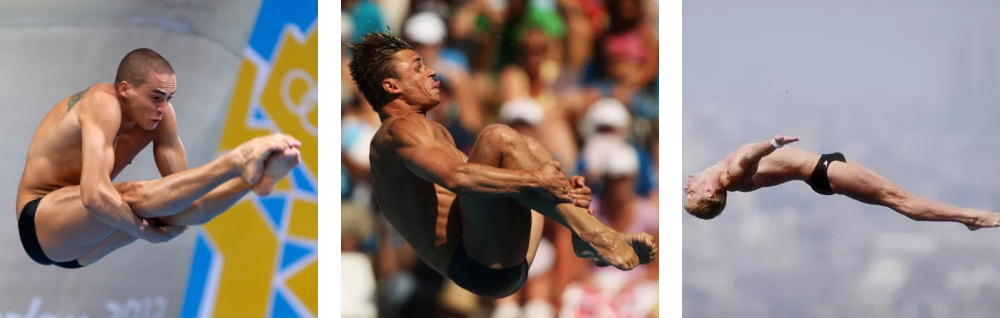
\includegraphics[scale=0.98]
{figures/dives.png}}
\caption{\label{fig:dive-styles} The figure shows the three main flight styles: pike, tuck, and straight respectively.}
\end{figure}

Our goal is to use spatio-temporal volumes to extract features that will then be used to train a convolutional neural network. This network will be used to classify previously unseen videos. Special importance will be placed in aggregating temporal data to solve possible short-term conflicts during the classification process, as the "pike" and "tuck" position can be confused for each other in certain angles. To train our network we plan to use the \textit{Diving48} dataset \cite{ref-diving48} which contains a large number of recordings from a variety of angles. All the videos in this dataset contain ground-truth labels that describe the sequence in four ways: (i) the type of takeoff, (ii) the number of somersaults, (iii) the number of twists, and (iv) the style of flight.

To simplify the extent of our work, we will remove the "free" flight style  from the dataset (i.e. the style where the performer combines several styles in one dive). Furthermore, we will clip the recordings to remove the parts where the performer sinks below the water. As a last preprocessing step, we will remove the performances with extreme camera angles. Afterwards, we will use the spatio-temporal volumes to extract features of interest (possibly legs and torso, as they can be easily segmented due to the separation provided by the swim trunk). Said features are represented as masks overlayed to the original video.

\section{Envisioned solution}

\subsection{Model - Processing Pipeline}
The two central frameworks used for this task are \emph{OpenCV} and \emph{TensorFlow}.

\subsubsection{Exctraction of Space-Time Volumes}
This step is performed by Filip Ilic and provides us - amongst others - with a three-dimensional tensor containing the STVs with unique identifier and the bounding box containing the diver.
\\
\textbf{TODO: Ask Filip what exactly the bounding box should contain, as it sometimes cuts some parts of the diver.}\\
\textbf{TODO: Ask Filip if the space-time volume identifier (value in the tensor) will be the same if the detection of a space-time volume was lost for a short time span.}

\subsubsection{STV Image Preprocessing}
As the algorithm for STV extraction occasionally provides small artefacts which do not relate to the diver, simple morphological operations might be beneficial the exclude them from further feature extraction. Nevertheless, most of these artefacts are outside of the bounding box anyway. Only the STVs within the bounding box are taken into account for further processing.

\subsubsection{Feature Extraction and Token Selection}
The token list should represent only the relavie motion of the diver, as the actual translational path of the diver does not provide any distinctive data for the individual classes. Moreover, it might even be misleading information, as the diving videos are taken from different perspectives and thus the translational path appears different on the two-dimensional image projection.\\
The intended token selection can be roughly divided into four sequential steps:
\begin{enumerate}
\item Selection of 2-3 largest (based on relative area w.r.t. bounding box) STVs in the bounding box, separately for each frame.
\item Contour extraction from the selected STVs, separately for each frame.
\item Fitting primitive two-dimensional shape to the selected STVs. One of the following shapes will be chosen during development:
  \begin{itemize}
  \item Minimum bounding rectangle (MBR)
  \item Ellipse
  \item Line
  \end{itemize}
\item Extracting scalar features based on the fitted shapes. The actual set of features which will be finally used, might be reduced based on principal component analysis.
  \begin{itemize}
  \item Absolute orientation angle
  \item Relative area with respect to bounding box
  \item Distance to the center of the bounding box
  \item Mutual relative orientation angle
  \item Mutual relative distance
  \item Elongation or aspect ratio
  \item Compactness
  \end{itemize}
\end{enumerate}

\subsubsection{Preprocessing in Feature Space}
Any angle in the token list is taken modulo $\pi$ and split up into it's sine and  cosine to ensure that similar orientation has similar feature values. The modulo operation represents that the fitted primitive 2D shape is symmetric (i.e. has no ``head'' and ``tail''). Moreover, the sine is multiplied by factor 2 and shifted by -1 to ensure the same range $[-1;1]$.\\
The area and distance features are scaled to the range $[-1;1]$ with respect to the bounding box of the current frame. To avoid detrimental effects resulting from flickering (i.e. rapid unrepresentative changes with time) of the bounding box, acausal average filtering is done over time.\\
\textbf{Median filtering?!}\\
\textbf{STV matching?!} Maybe opencv flann nearest neighbor search

\subsubsection{Classification}
The actual classification task will be performed by learning a convolutional neural network. The convolution layers will consist of one-dimensional convolutions, separately for each scalar feature. Additionally, there will be moderate pooling layers. The cross entropy is taken as cost function.

\section{Expected results}

\subsection{Potential Difficulties}
\begin{itemize}
\item STV discontinuities in time; means taking wrong/non-descriptive 2-3 largest STVs; this means mixing up (blockwise) the values in the feature vector, which might confuse the NN
\item Bounding box cutting STVs means possible exclusion of descriptive STVs
\end{itemize}

\bibliography{references/references.bib}

\end{document}
